\documentclass[12pt]{article}
\usepackage{latexsym}
\usepackage[activeacute,spanish]{babel}
\usepackage{graphicx}
\graphicspath{ {images/} }

\title{Tutorial\\Iniciando con Struts2, Hibernate y Spring\\Usando Sitemesh como proveedor de estilo\\y maven como manejador de scripts}
\author{Smart Software Development for Enterprises\\jorge.rivera@ssde.com.mx}

\begin{document}
\maketitle
\newpage
\tableofcontents
\newpage
\listoffigures
\newpage

    \section{Introducci\'on}
		Este tutorial est\'a basado en en tutorial de Chris Hulbert.
		\\
		En este tutorial usaremos maven como el proveedor de scripts para inicializaci\'on y compilaci\'on as\'i como tambi\'en administrar las librerias y las versiones de las mismas.

		\subsection{Requerimientos}
		Para este tutorial utilizaremos:
		\begin{itemize}
		\item Eclipse (Puede usarse cualquier otro IDE o editor de texto)
		\item Tomcat 7 (Puede usarse una versi\'on m\'as reciente)
		\item Maven 3.3.9
		\item JDK 1.7 (Puede usarse una versi\'on m\'as reciente)
		\item git 2.10.1 (Puede usarse otro repositorio)
		\end{itemize}

		\subsection{Creando nuestro proyecto}
		Hay varias formas de crear nuestro proyecto, una de ellas es por medio de la consola (l\'inea 
		de comandos, terminal, etc.) otra es usando alguno de los IDEs disponibles, Eclipse, IntelliJ,
		 etc.
		\\Enseguida mostraremos como hacerlo:

		\subsubsection{Terminal}
		
		Abrimos nuestra terminal, previamente hemos instalado Maven y JDK, nos posicionamos en el folder
		en el que nuestro proyecto va a residir y tecleamos:\\
		\linebreak
		\texttt{mvn archetype:generate -DgroupId=com.ssde.tutorial -DartifactId=test -DarchetypeArtifactId=maven-archetype-webapp -DinteractiveMode=false}\\
		\linebreak
		\textbf{Que significan todos esos parametros?}

		\begin{description}
		\item [archetype:generate] Le dice a mvn que vamos a utilizar un arquetipo para generar nuestra aplicaci\'on.
		\item[-DgroupId=com.ssde.tutorial] Designa com.ssde.tutorial como el paquete principal para nuestra aplicacion.
		\item[-DartifactId=test] Designa test como el nombre de nuestra aplicacion.
		\item[-DarchetypeArtifactId=maven-archetype-webapp] Es el nombre del arquetipo a utilizar por maven para crear el proyecto
		\item[-DinteractiveMode=false] Le dice a mvn que no necesita interacci\'on del usuario.
		\end{description}
		\subsubsection{Eclipse}
		
		Abrimos Eclipse, vamos al men\'u "Nuevo...", seleccionamos "Proyecto..." y buscamos la categor\'ia Maven y seleccionamos Proyecto Maven como se ve en la figura \ref{01_nuevo_proyecto}
        \begin{figure}[h]
            \centering
            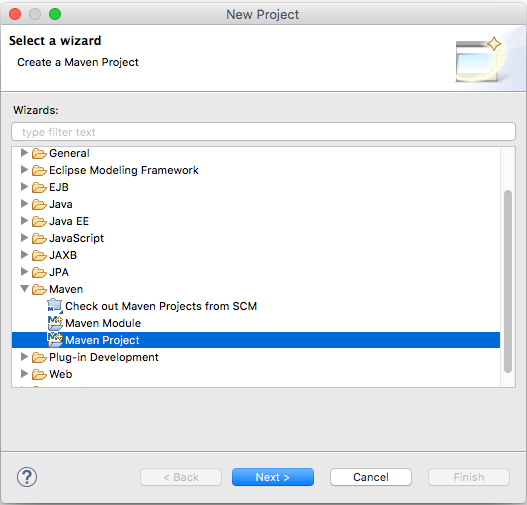
\includegraphics[scale=0.4]{01_nuevo_proyecto}
            \caption{Proyecto Maven}
            \label{01_nuevo_proyecto}
        \end{figure}
		\\
		En la siguiente ventana como se muestra en la figura \ref{02_nuevo_proyecto}, asegurate de NO seleccionar ''Crear proyecto simple (saltar selecci\'on de arquetipo)", presionamos siguiente...
        \begin{figure}[h]
            \centering
            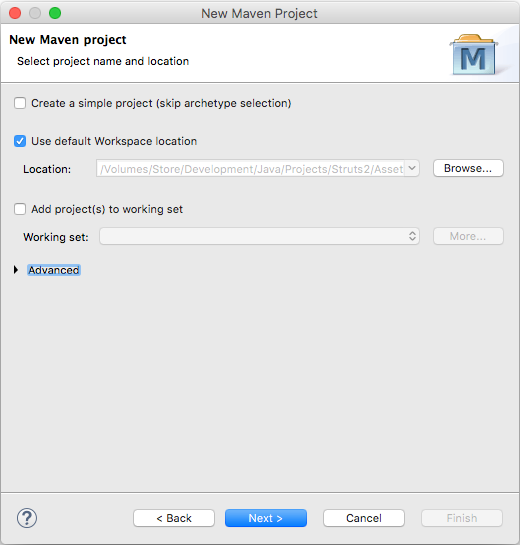
\includegraphics[scale=0.4]{02_nuevo_proyecto}
            \caption{Seleci\'on del folder donde guardar el proyecto}
            \label{02_nuevo_proyecto}
        \end{figure}
        \\
        En la nueva ventana, figura \ref{03_nuevo_proyecto}, veremos la lista de los arquetipos disponibles, regularmente el que necesitamos \texttt{maven-archetype-webapp}, una vez seleccionada presionamos siguente...
         \begin{figure}[h]
            \centering
            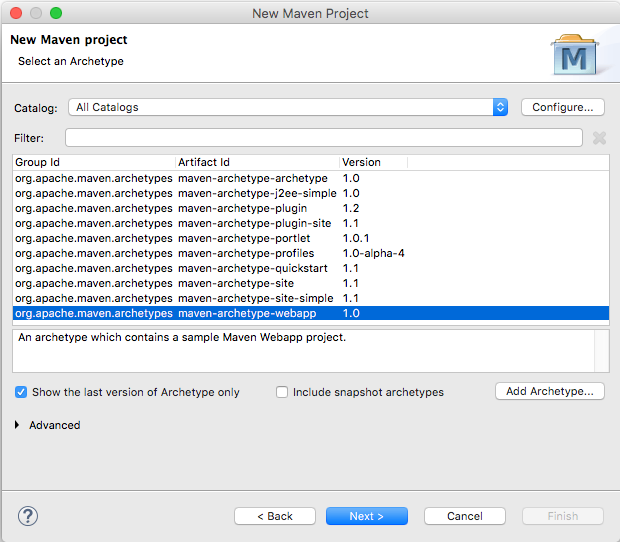
\includegraphics[scale=0.4]{03_nuevo_proyecto}
            \caption{Selecci\'on del arquetipo}
            \label{03_nuevo_proyecto}
        \end{figure}
        \\
        En \'esta \'ultima ventana, figura \ref{04_nuevo_proyecto}, podemos definir el nombre de nuestra aplicaci\'on y el nombre del paquete al que pertenecer\'a, una vez elegido esto podemos terminal el Wizard y tendremos nuestro esqueleto de aplicaci\'on listo para empezar a trabajar.
        \begin{figure}[h]
            \centering
            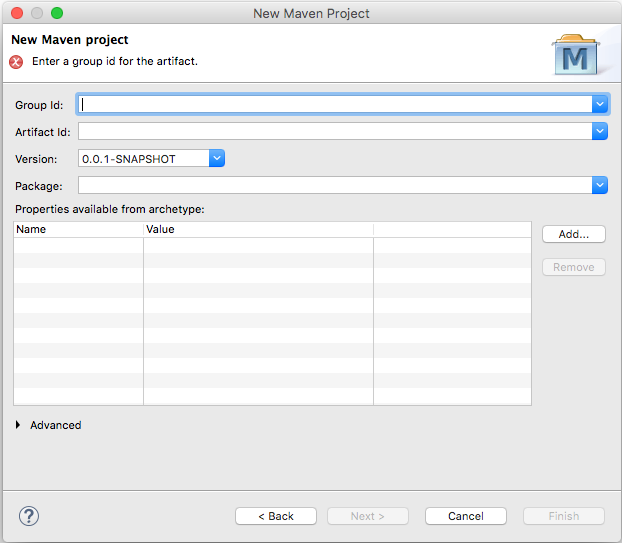
\includegraphics[scale=0.4]{04_nuevo_proyecto}
            \caption{Detallando los paquetes y el nombre de la aplicaci\'on}
            \label{04_nuevo_proyecto}
        \end{figure}
        \newpage
        
		\subsection{Instalando Tomcat}
		Descargamos de el sitio de apache https://tomcat.apache.org/download-70.cgi, una vez descargado el arvhivo zip, lo colocamos en un folder para de ah\'i iniciar el servidor.\\
		Vamos al folder conf dentro de tomcat y modificamos el archivo tomcat-users.xml para agregar los roles admin, admin-gui y manager-gui, agregamos un usuario asignamos una contrasena y le asignamos dichos roles. Eso es todo, tomcat est\'a listo para ser utilizado.
		\newpage

    \section{Sitemesh}
		Utilizaremos Sitemesh como el proveedor de tema para nuestra aplicaci\'on, primero necesitamos agregar la dependencia a nuestro archivo pom.xml, para este tutorial utilizaremos la versi\'on m\'as reciente de sitemesh 3.0.1.\\
		\subsection{pom.xml}
		Es com\'un agregar un apartado de propiedades al archivo pom.xml donde especificamos las versiones de nuestras librer\'ias, justo debajo de la especificaci\'on inicial de nuestra aplicaci\'on, como se muestra en la figura \ref{05_pom_xml}.
        \begin{figure}[h]
            \centering
            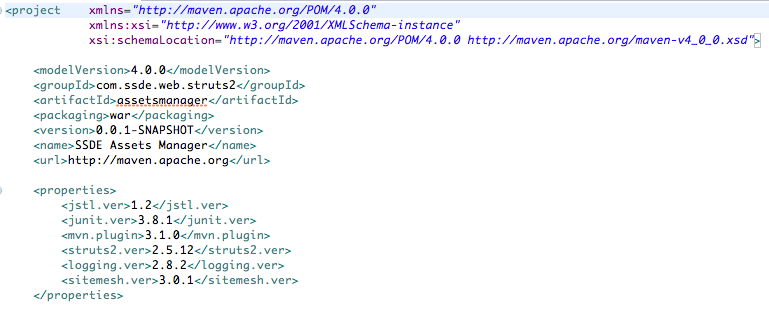
\includegraphics[scale=0.4]{05_pom_xml}
            \caption{Localizaci\'on de el bloque de propiedades en el archivo pom.xml}
            \label{05_pom_xml}
        \end{figure}
        
        Una vez definida la version de nuestra librer\'ia agregamos la dependencia en el bloque de dependencias como se muestra en la figura \ref{06_pom_xml}
        \begin{figure}[h]
            \centering
            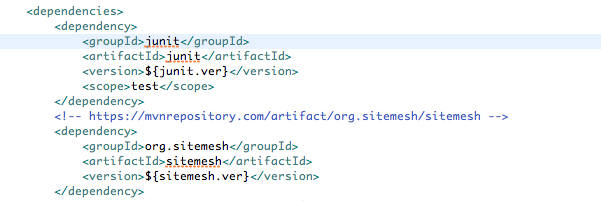
\includegraphics[scale=0.4]{06_pom_xml}
            \caption{Agregando la dependencia de Sitemesh}
            \label{06_pom_xml}
        \end{figure}
        \newpage
        
        \subsection{web.xml}
        Es tiempo de agregar Sitemesh a nuestro archivo web.xml, como se describe en la figura \ref{07_web_xml}, este bloque debe estar al fondo de nuestro archivo web.xml
        \begin{figure}[h]
            \centering
            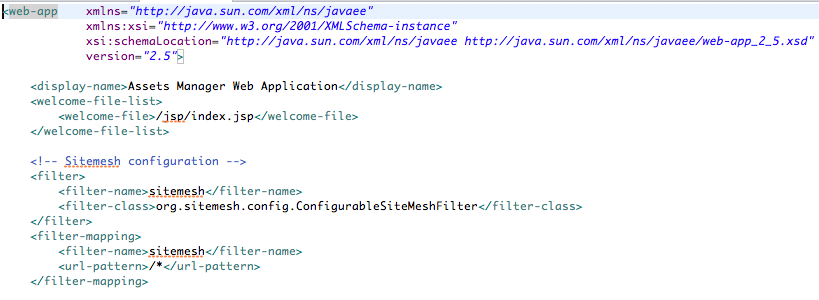
\includegraphics[scale=0.4]{07_web_xml}
            \caption{Agregando el filtro para Sitemesh}
            \label{07_web_xml}
        \end{figure}
        \newpage
        
        \subsection{sitemesh3.xml}
        Para designar nuestra plantilla para el tema a utilizar necesitamos agregar el archivo sitemesh3.xml en el mismo folder que nuestro archivo web.xml est\'a situado, el contenido de dicho archivo se muestra en la figura \ref{08_sitemesh3_xml}.
        \begin{figure}[h]
            \centering
            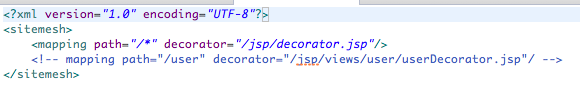
\includegraphics[scale=0.4]{08_sitemesh3_xml}
            \caption{Agregando el archivo decorador de Sitemesh y su localizaci\'on}
            \label{08_sitemesh3_xml}
        \end{figure}
        \newpage
        
        \subsection{decorator.jsp}
        La figura \ref{09_decorator_jsp} nos muestra la configuraci\'on m\'inima para nuestro archivo decorador, se puede utilizar tambi\'en el archivo main.jsp que Chris Hulbert usa en su tutorial junto con la hoja de estilos y las im\'agenes que utiliza
        \begin{figure}[h]
            \centering
            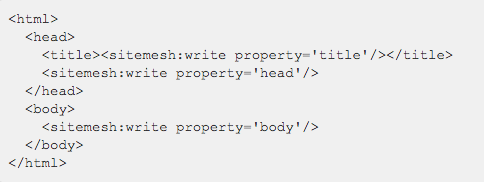
\includegraphics[scale=0.7]{09_decorator_jsp}
            \caption{Configuraci\'on m\'inima del archivo decorador}
            \label{09_decorator_jsp}
        \end{figure}
        
        Para probar que sitemesh est\'a funcionando podemos compilar nuestro proyecto y crear el archivo contendor (proyecto.war) y desplegarlo en nuestro servidor tomcat ustilizando el manejador de aplicaciones http://localhost:8080/manager/html. Hasta este punto si todo ha ido bien, veremos la imagen que se muestra en la figura \ref{10_tomcat_sitemesh}
        \begin{figure}[h]
            \centering
            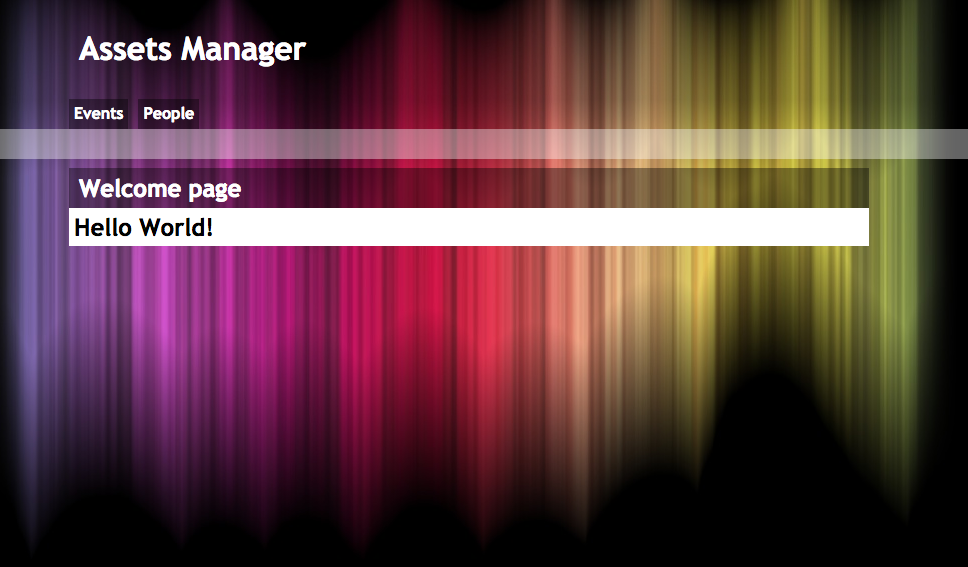
\includegraphics[scale=0.4]{10_tomcat_sitemesh}
            \caption{Sitemesh funcionando como nuestro manejador de tema}
            \label{10_tomcat_sitemesh}
        \end{figure}
		\newpage

    \section{Struts 2}
    \newpage
		\subsection{uno}
		\newpage
		\subsection{dos}
		\newpage
		\subsection{tres}
		\newpage

    \section{Logging}
    \newpage
		\subsection{Ingresos}
		\newpage
		\subsection{Gastos}
		\newpage
		\subsection{Proveedores}
		\newpage

    \section{Spring}
    \newpage
		\subsection{uno}
		\newpage
		\subsection{dos}
		\newpage
		\subsection{tres}
		\newpage


    \section{Hibernate}
    \newpage
		\subsection{uno}
		\newpage
		\subsection{dos}
		\newpage
		\subsection{tres}
		\newpage

    \section{Preguntas frecuentes}
    \newpage
		\subsection{uno}
		\newpage
		\subsection{dos}
		\newpage
		\subsection{tres}
		\newpage

\end{document}